%%%%%%%%%%%%%%%%%%%%%%%%%%%%%%%%%%%%%%%%%%%%%%%%%%%%%%%%%%%%%%%%%%%%%%%%%%%%%%%%%%%%%%%%%%
\section{Results}

%%%%%%%%%%%%%%% Parameters %%%%%%%%%%%%%%%
% n_data = 20 - n_data in x and y: n_tot = 20*20
% test_size = 0.2
% noise = 0.2 - aptitude of normal distributed noise    
% data_dim = 2

%%%%%%%%%%%%%%% Part b %%%%%%%%%%%%%%%
% * Evaluate MSE up to 5.th order fro OLS. 
% * and R2 score
% * blot parameters beta
% * Your code has to include a scaling/centering:
%   XXX: not included, data is already scaled in intervall [-1, 1]

\begin{figure}[H]
    \centering
    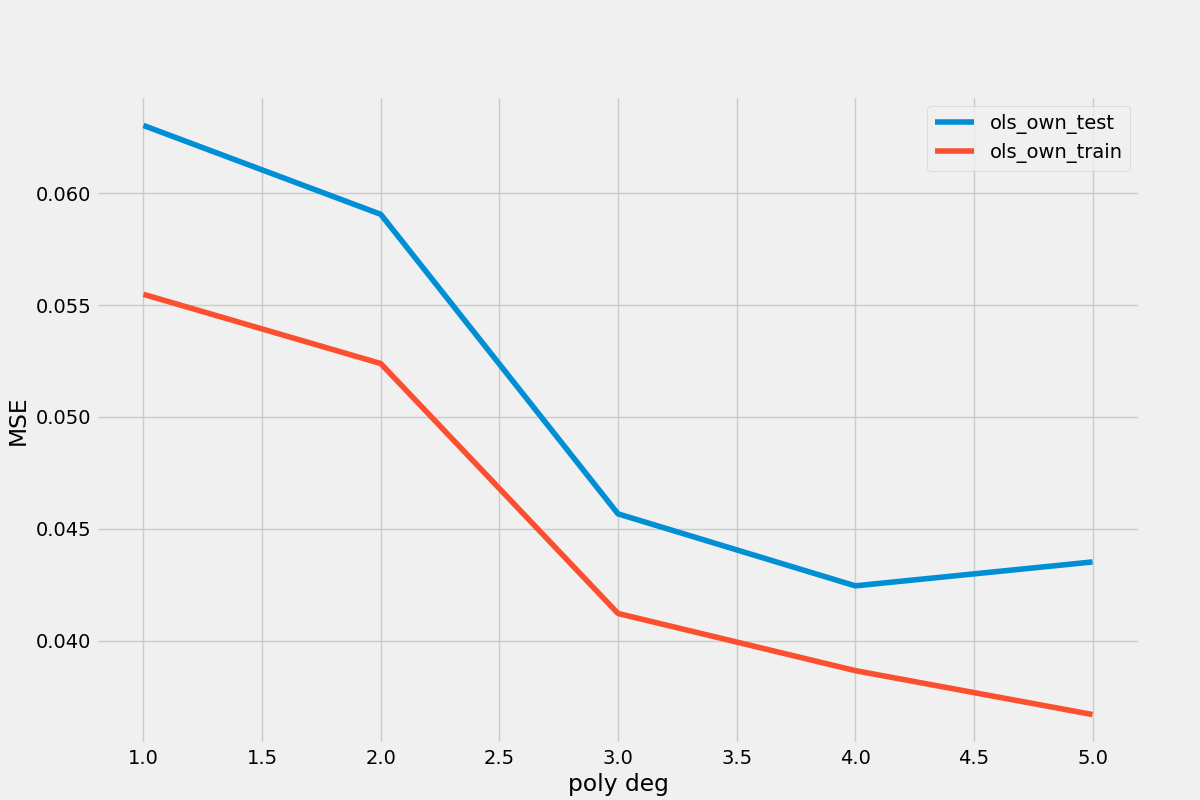
\includegraphics[width=0.8\textwidth]{Figures/b_mse.png}
\end{figure}

\begin{figure}[H]
    \centering
    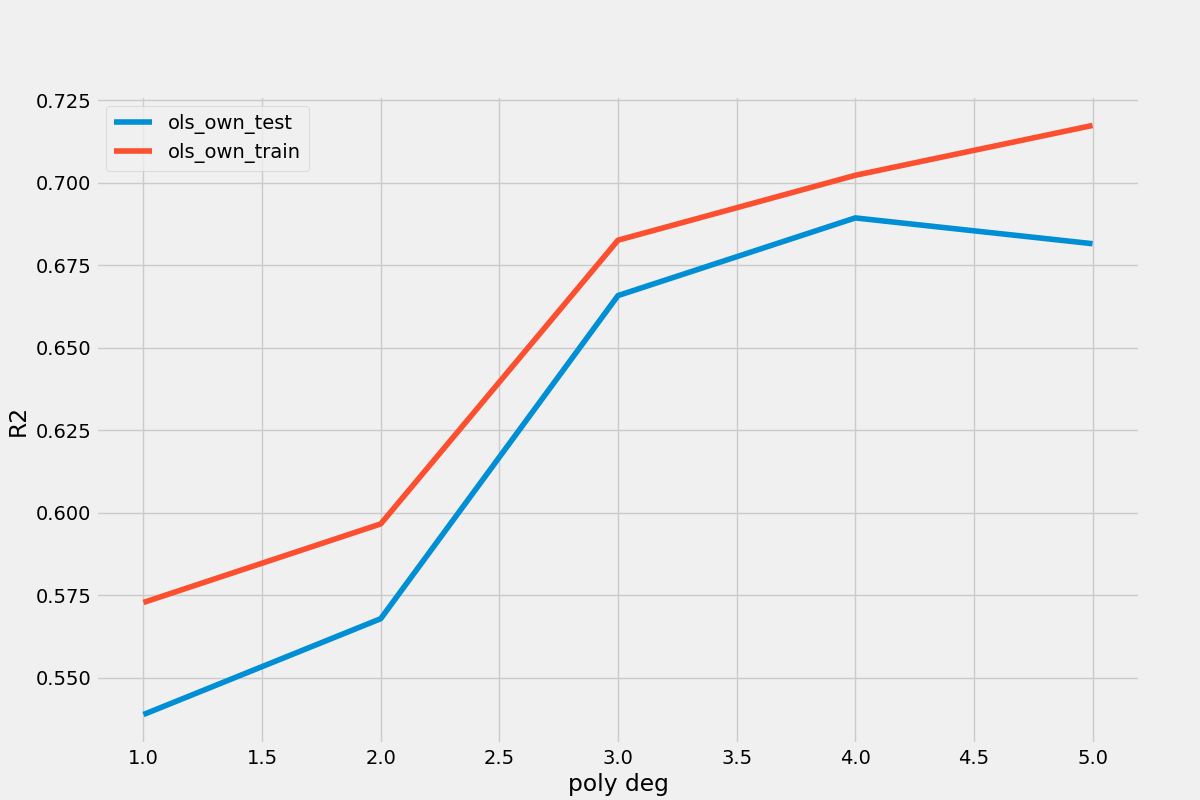
\includegraphics[width=0.8\textwidth]{Figures/b_r2.png}
\end{figure}

% TODO: error bars
\begin{figure}[H]
    \centering
    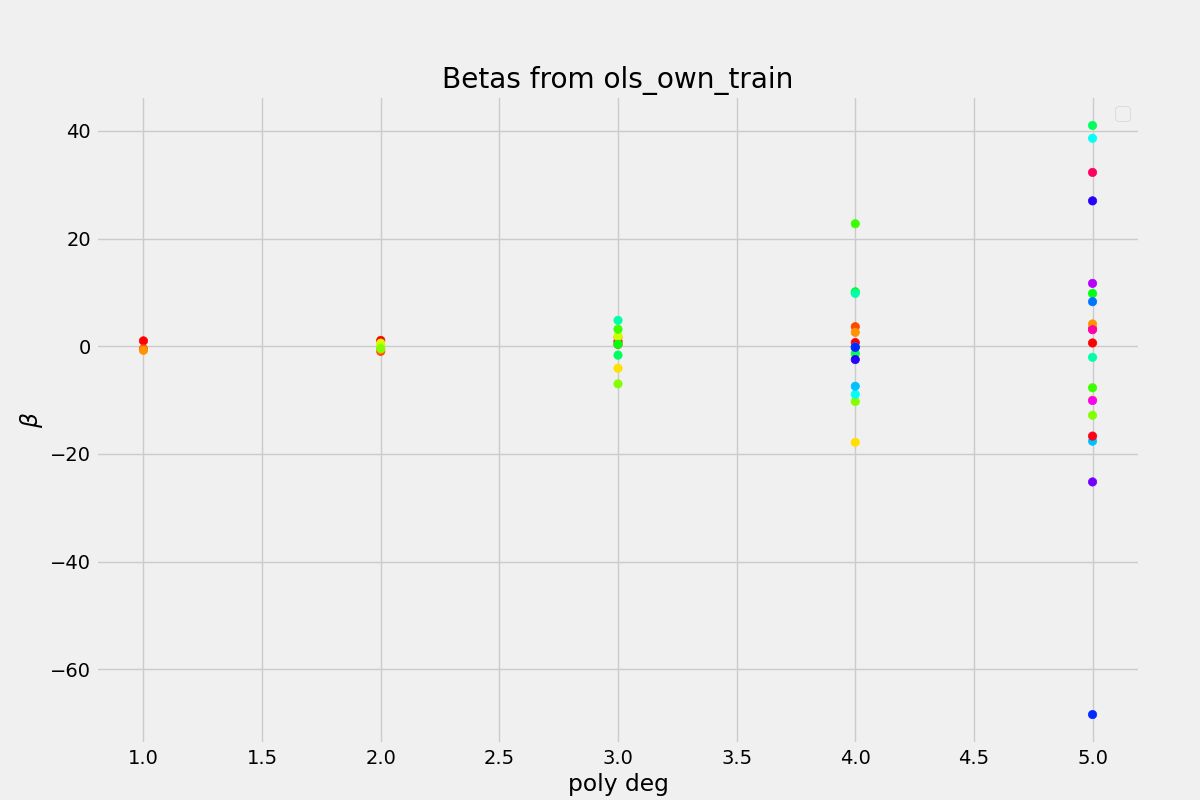
\includegraphics[width=0.8\textwidth]{Figures/b_beta.png}
\end{figure}





%%%%%%%%%%%%%%% Part c  %%%%%%%%%%%%%%%



$R^2$ and MSE plot of OLS, Ridge and lasso
